\section{Experiments}

\subsection{Cartesian Lattice}
Blurb about cartesian lattices.

\subsubsection{Basis function}
Choosing $\mathbf{\Xii = \Xii_{C2} := \left[ I_3  \ I_3 \right]}$ (the $3 \times 6$ matrix created by the union of two identity matrices) generates a triliniear piecewise polynomial. It is easy to see, by definition, when $\mathbf{\Xii_{C2}}$ is used in conjunction with \EQp{eq:box_def}, the resulting function $M_\mathbf{\Xii_{C2}}(\vx)$ corresponds to the non-centered tensor product extension of the linear B-spline in three dimensions. Likewise, the non-centered cubic tensor product box spline is given by $M_\mathbf{\Xii_{C4}}(\vx)$, where $\mathbf{\Xii_{C4} := \left[ I_3  \ I_3 \ I_3  \ I_3 \right]}$. A box spline is easily centered by taking $M_\mathbf{\Xii}(\vx + \mathbf{c_\Xii})$, with $\mathbf{c_\Xii}:=\sum_{\xi \in \mathbf{\Xii}} \frac{1}{2}\xi$. We will assume, unless otherwise stated, that $M_\mathbf{\Xii}$ defines the centered box spline generated by $\mathbf{\Xii}$.

\subsubsection{Filter weights}


\subsection{BCC Lattice}
Blurb about cartesian lattices.

\subsubsection{Basis function}
On the BCC lattice, a choice of {\footnotesize
\begin{equation*}
	\mathbf{\Xii_{B}} := 
	\begin{bmatrix} 
		-1 & 1 & 1 & -1 \\
		1 & -1 & 1 & -1 \\
		1 & 1 & -1 & -1 
	\end{bmatrix}
\end{equation*}}

generates a piecewise linear polynomial function \cite{practicalbox}. The support of this box spline is a rhombic dodecahedron, which incidentally contains the set of first nearest neighbors to the Voronoi region of the lattice at the origin, and is a natural fit for the lattice. The quintic box spline is given by the matrix $\mathbf{\Xii_{B2}} := \left[\mathbf{\Xii_{B}} \ \mathbf{\Xii_{B}}\right]$, or may also be seen as the convolution of the linear box spline with itself.  However, there exist both an efficient piecewise polynomial representation \cite{practicalbox}, and an efficient implementation \cite{fastbox} of these piecewise quintic polynomial functions.

\subsubsection{Filter weights}


\subsection{Shifted Basis Functions}
We also consider shifted box splines $M_{\mathbf{\Xii}}^{\xi_i}(\vx) := M_{\mathbf{\Xii}}(\vx - \frac{1}{2}\mathbf{\xi}_i)$, where $\mathbf{\xi}_i$ is any direction vector in $\mathbf{\Xii}$. In the univariate case with linear B-splines, it has been shown that introducing a shift can offer an improvement when representing scalar data \cite{linearrev}. More generally and relevant to our purposes, they have also been shown to reduce error when approximating the gradient of scalar fields \cite{gradrev}.

\begin{table}[!t]
	%% increase table row spacing, adjust to taste
	\renewcommand{\arraystretch}{1.5}
	% if using array.sty, it might be a good idea to tweak the value of
	%\extrarowheight % as needed to properly center the text within the cells
	\centering
	% Some packages, such as MDW tools, offer better commands for making tables
	% than the plain LaTeX2e tabular which is used here.
	\begin{tabular}{|r||c||c|c|}
		\hline
		Filter & Notation & Filter wieghts  \\
		\hline
		\hline
		Derivative & $d[n]$ & $[\frac{-1}{12} \ \frac{2}{3} \ 0 \ \frac{-2}{3} \ \frac{1}{12}]$ \\
		\hline
		Shifted Derivative & $s[n]$  & $[\frac{-1}{24} \ \frac{9}{8} \ \frac{-9}{8} \ \frac{1}{24} \ 0]$ \\
		\hline
		Second Derivative & $l[n]$  & $[\frac{-1}{12} \ \frac{4}{3} \ \frac{-5}{2} \ \frac{4}{3} \ \frac{-1}{12}]$ \\
		\hline
	\end{tabular}
	\caption{Filters used in our experiments. These filters are applied along the principal lattice directions.}
	\label{tab:filters}
\end{table}

\section{Results and Discussion}
For our tests, we restrict ourselves to the function spaces spanned by the Cubic tensor product basis on the Cartesian lattice, and the Quintic basis function on the BCC lattice. To provide a baseline reconstruction with which to compare our results, we consider FFT, Poisson and Screened Poisson Methods. We utilize the test models and point-sets of the Anchor, Daratech, Dancing Children, Gargoyle, and Quasimoto models provided by the Surface Reconstruction Benchmark \cite{reconbench}.

Quantitatively, we evaluate whether function spaces on the BCC lattice provide better approximation spaces than those on the Cartesian lattice. In order to reduce any artifacts that may arise from any noise or the non-uniformity of the data, we utilize the ideal reference point-sets of our test models.  We measure both the Hausdorff distance, mean distance, and angle deviation from the original shape with the tools provided by Berger et al.~\cite{reconbench}. We evaluate the FFT, Poisson, and Screened Poisson surface reconstruction algorithms, as their theory is close to ours. We choose $\lambda_1$ and $\lambda_2$ so that the reconstructions are comparable to the Screened Poisson results.

Since the Gargoyle model has many interesting high frequency features, we consider reconstructing it at increasing grid resolutions. For the Poisson and Screened Poisson methods, we restrict the depth of the tree so that the finest resolution provided by the oct-tree is equivalent to that of the regular Cartesian, \FG{fig:t1}. We also seem to be able to improve upon the Screened Poisson method, however, the parameter space needs to be explored further to conclusively assert this. Regardless, it is still a good baseline with which to compare our results. 

%You should really try to bring out the role of the shifts.
We fix the resolution of the grid at $128^3$, and reconstruct the remaining models (\FG{fig:t2}.) We choose this resolution as it seems to be a point of contention between the cases with the Gargoyle model. However, there seems to be a consistent advantage in using the BCC lattice over the Cartesian lattice. Moreover, in both cases, we noticed that introducing a shift tends to reduce all error metrics. Unfortunately, reconstructing the divergence of the smoothed vector field from more than three lattice directions produced little difference. \FG{fig:r1} shows a visual comparison of the techniques. We manage to outperform the FFT and Poisson techniques by a large margin, and outperform the screened Poisson case.

\begin{figure*} 
	\centering
	\begin{tabular}{c c c c}
	\includegraphics[width=0.23\linewidth]{figures/dist32.eps} &
	\includegraphics[width=0.23\linewidth]{figures/dist64.eps} &
	\includegraphics[width=0.23\linewidth]{figures/dist128.eps} &
	\includegraphics[width=0.23\linewidth]{figures/dist256.eps} \\
	\includegraphics[width=0.23\linewidth]{figures/angle32.eps} &
	\includegraphics[width=0.23\linewidth]{figures/angle64.eps} &
	\includegraphics[width=0.23\linewidth]{figures/angle128.eps} &
	\includegraphics[width=0.23\linewidth]{figures/angle256.eps} 
	\end{tabular}
	\caption{An error comparison for the Gargoyle model as the grid resolution increases from $32^3$ to $256^3$ in steps of powers of two. The top row represents the Hausdorff (bar height) and mean distance (black line) to the original baseline model, while the bottom row represents the max angle deviation. $\lambda_1 = 100$, and $\lambda_2$, was chosen to be $1\scint{-3}$, $1\scint{-4}$, $1\scint{-5}$ and $1\scint{-6}$ from left to right respectively. Notice that the introduced shift greatly reduces angular error.}
	\label{fig:t1}
\end{figure*}

\begin{figure*} 
	\centering
	\begin{tabular}{c c c c}
	\includegraphics[width=0.23\linewidth]{figures/anchor/_dist.eps} &
	\includegraphics[width=0.23\linewidth]{figures/daratech/_dist.eps} &
	\includegraphics[width=0.23\linewidth]{figures/dc/_dist.eps} &
	\includegraphics[width=0.23\linewidth]{figures/quasimoto/_dist.eps} \\

	\includegraphics[width=0.23\linewidth]{figures/anchor/_angle.eps} &
	\includegraphics[width=0.23\linewidth]{figures/daratech/_angle.eps} &
	\includegraphics[width=0.23\linewidth]{figures/dc/_angle.eps} &
	\includegraphics[width=0.23\linewidth]{figures/quasimoto/_angle.eps} \\
	Anchor & Daratech & Dancing Children & Quasimoto 
	\end{tabular}
	\caption{A similar comparison for the case in which the grid is fixed at a resolution of $128^3$ for all models. Here, $\lambda_1=1\scint{2}$, and $\lambda_2=5\scint{-5}$. Again, we see the same trend of the BCC lattice outperforming the comparable Cartesian lattices, and the Screened Poisson approach.}
	\label{fig:t2}
\end{figure*}

\begin{figure} 
	\centering
	\begin{tabular}{c c}
		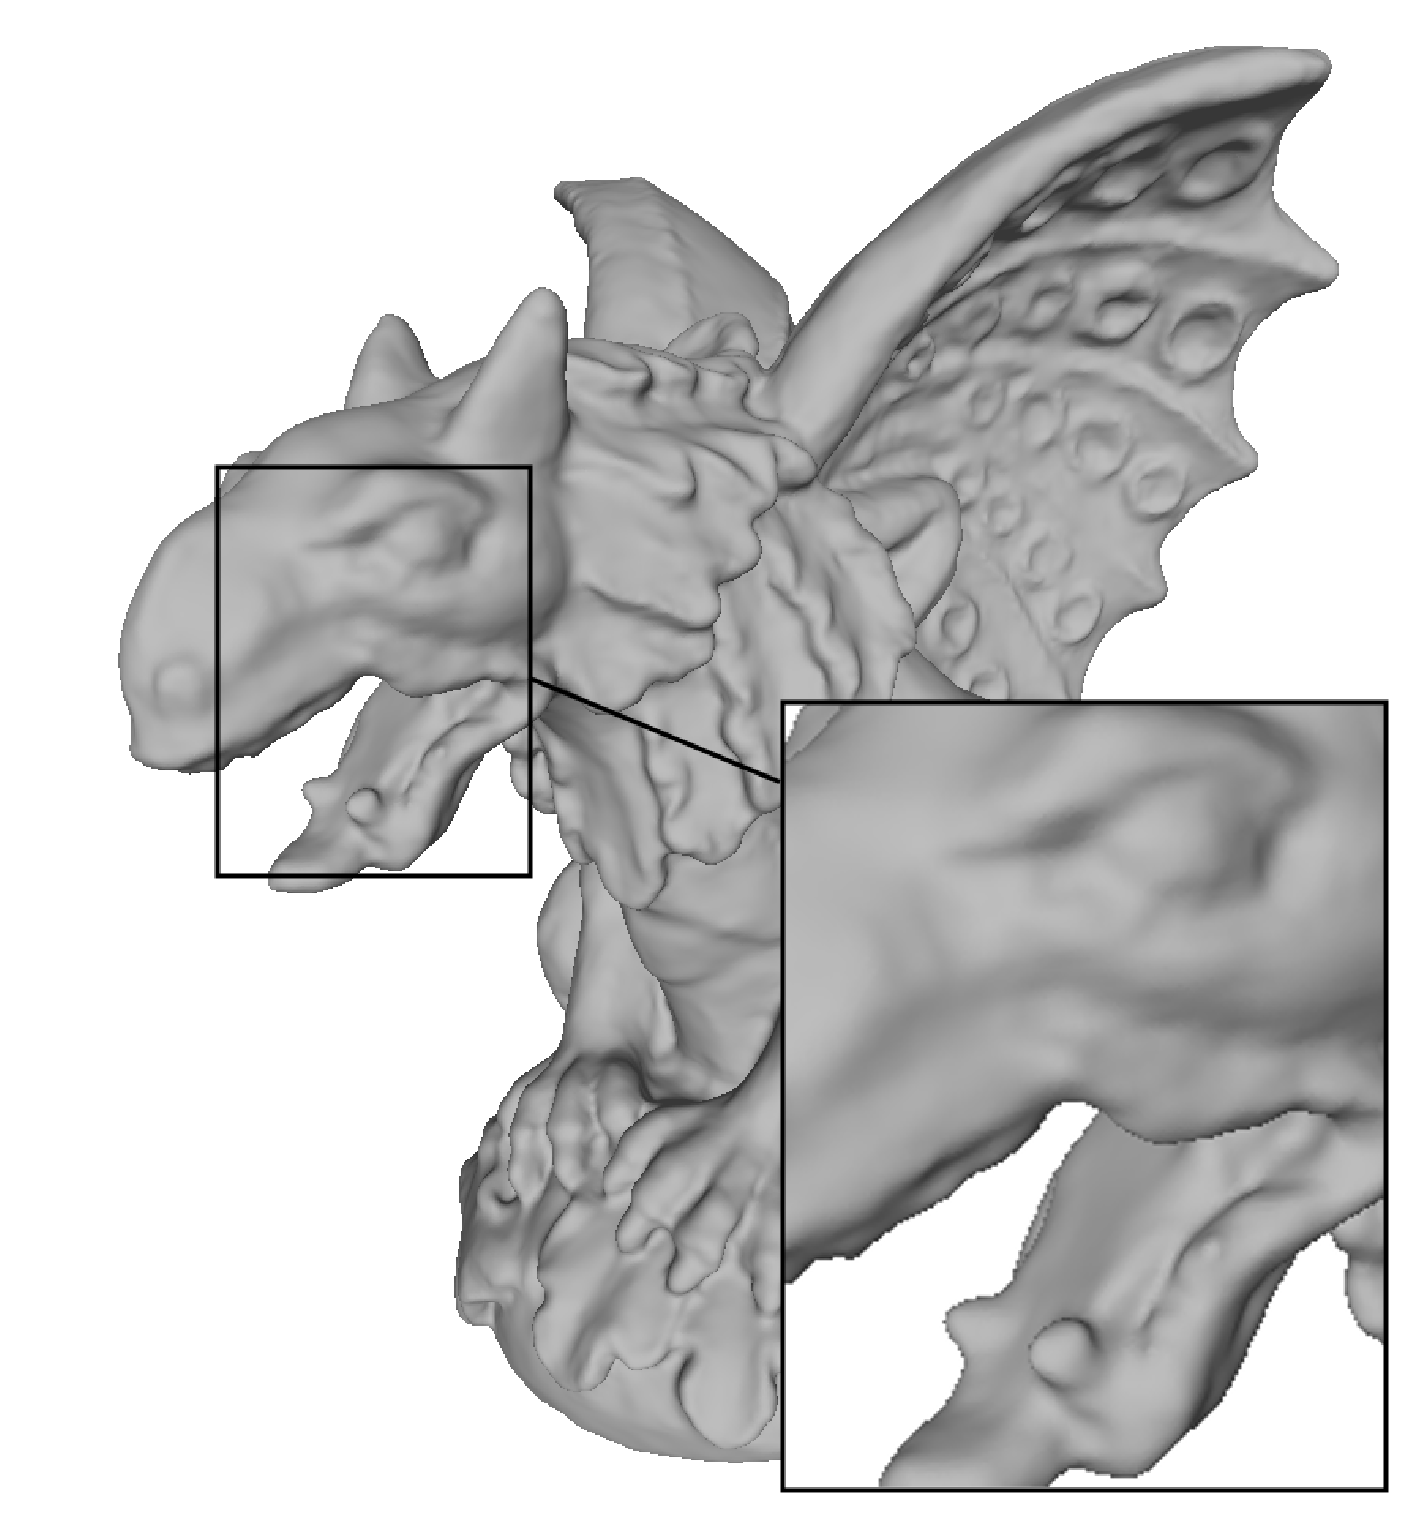
\includegraphics[width=0.48\linewidth,natwidth=750,natheight=750]{images/gargoyle/original.eps} &
		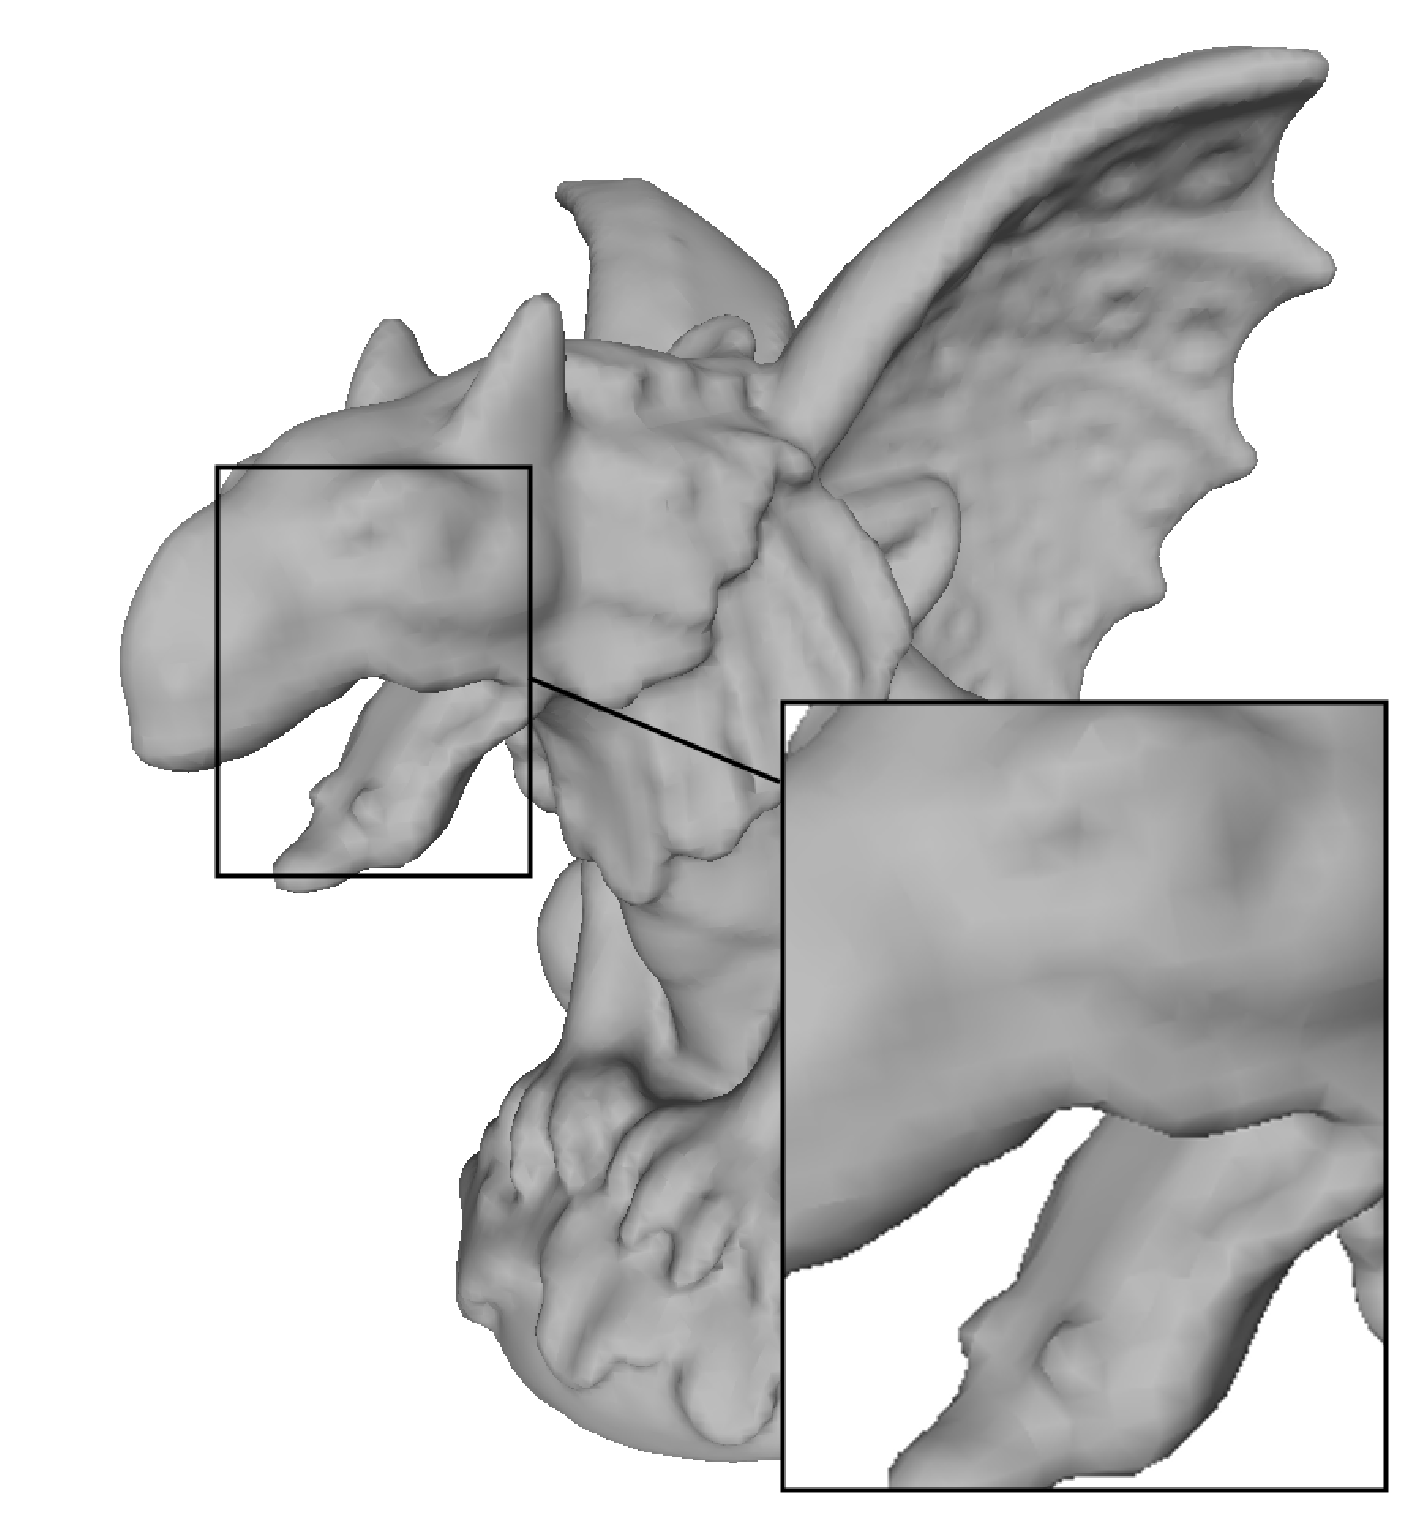
\includegraphics[width=0.48\linewidth,natwidth=750,natheight=750]{images/gargoyle/poisson.eps} \\
		Original & Poisson \\
		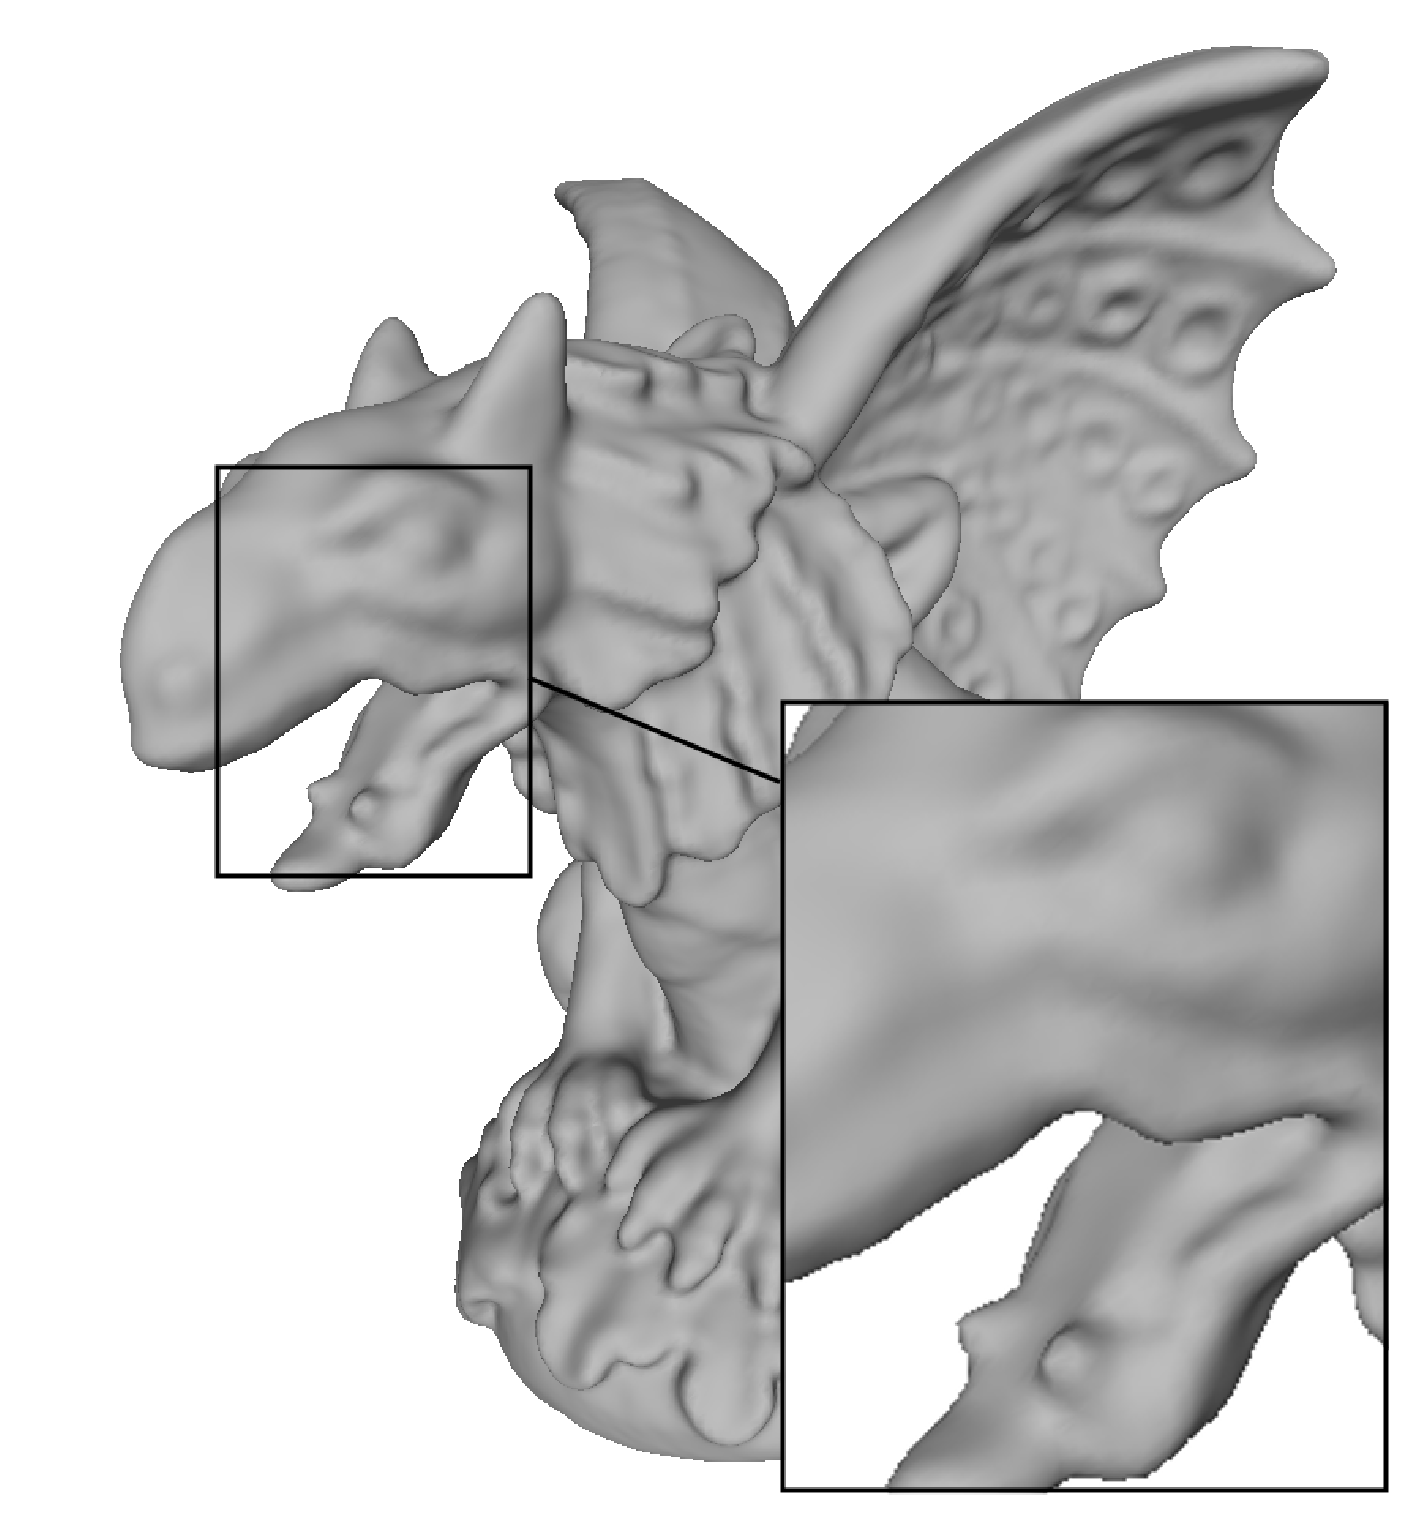
\includegraphics[width=0.48\linewidth,natwidth=750,natheight=750]{images/gargoyle/bcc.eps} &
		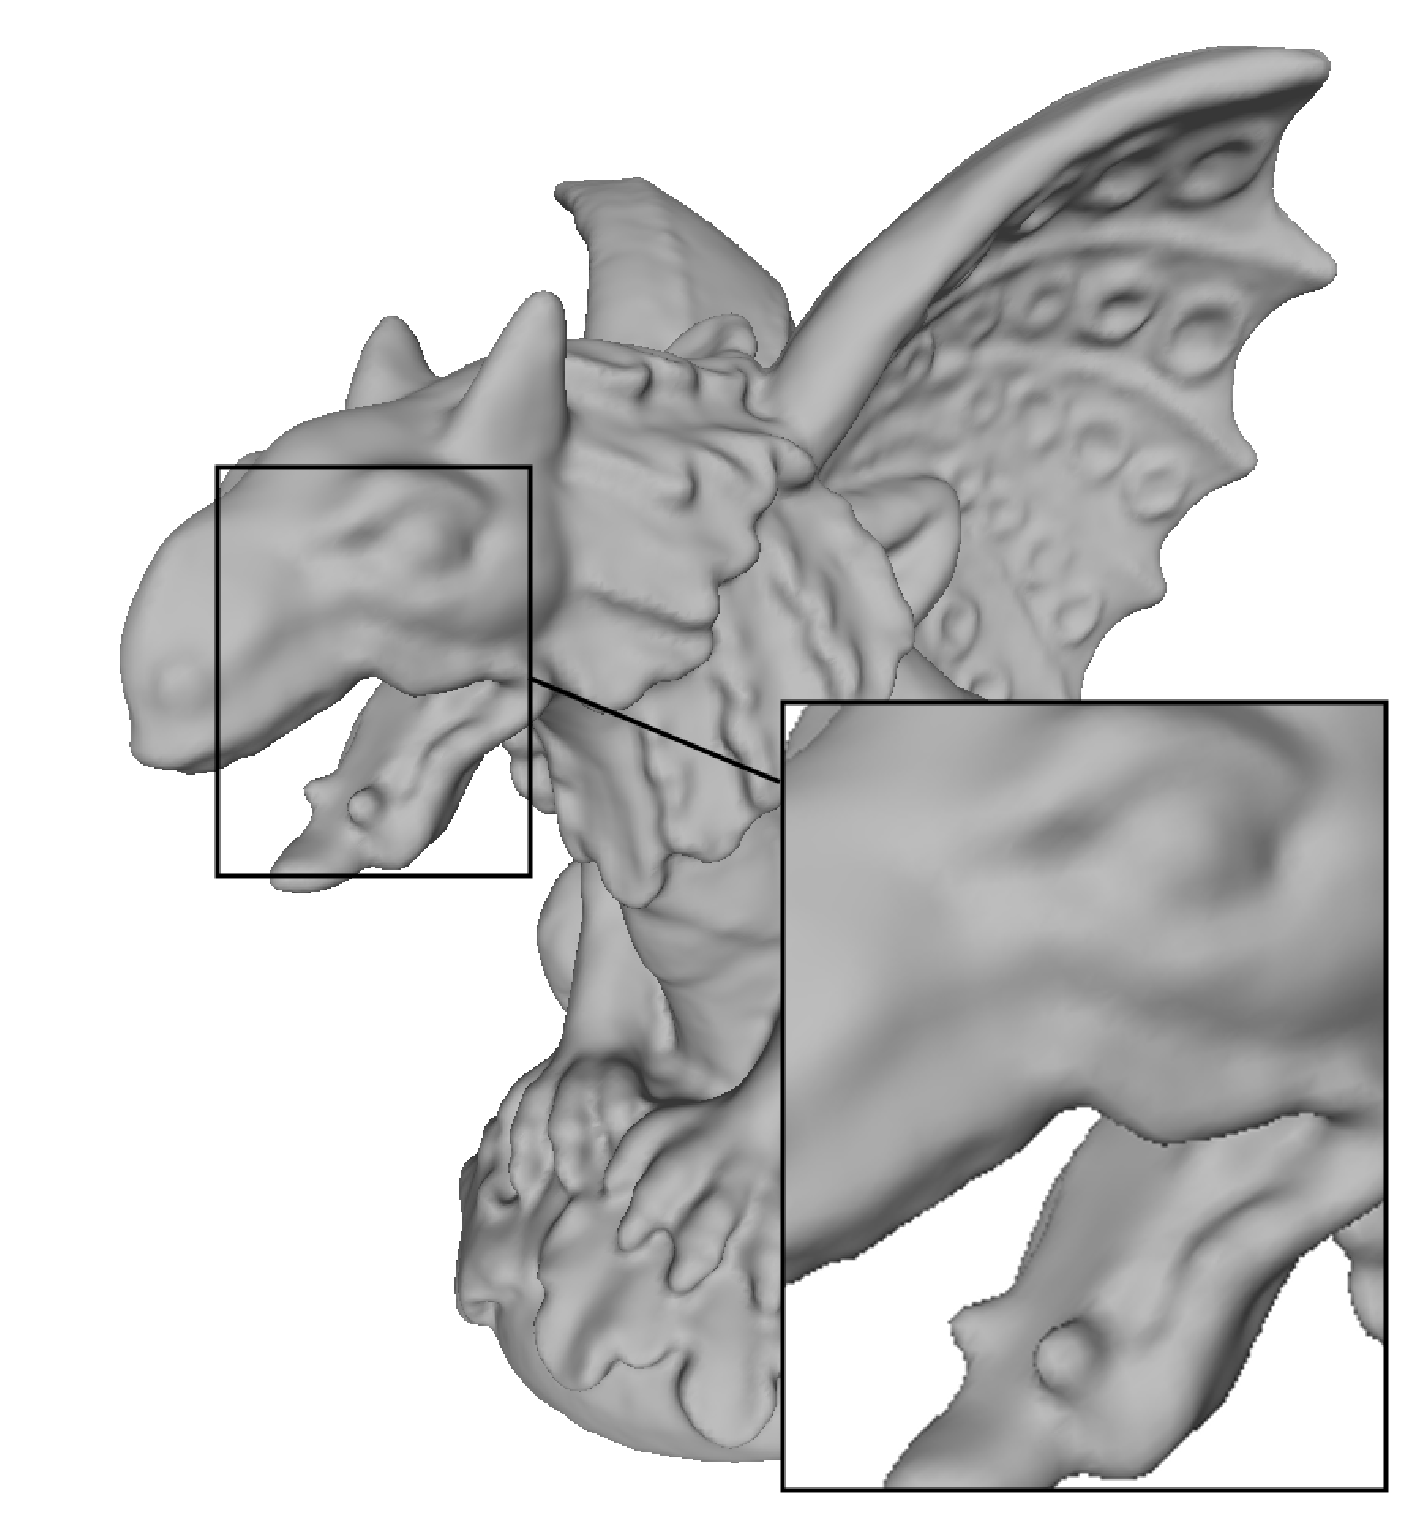
\includegraphics[width=0.48\linewidth,natwidth=750,natheight=750]{images/gargoyle/bccs.eps} \\ 
		BCC & BCC Shifted \\ 
		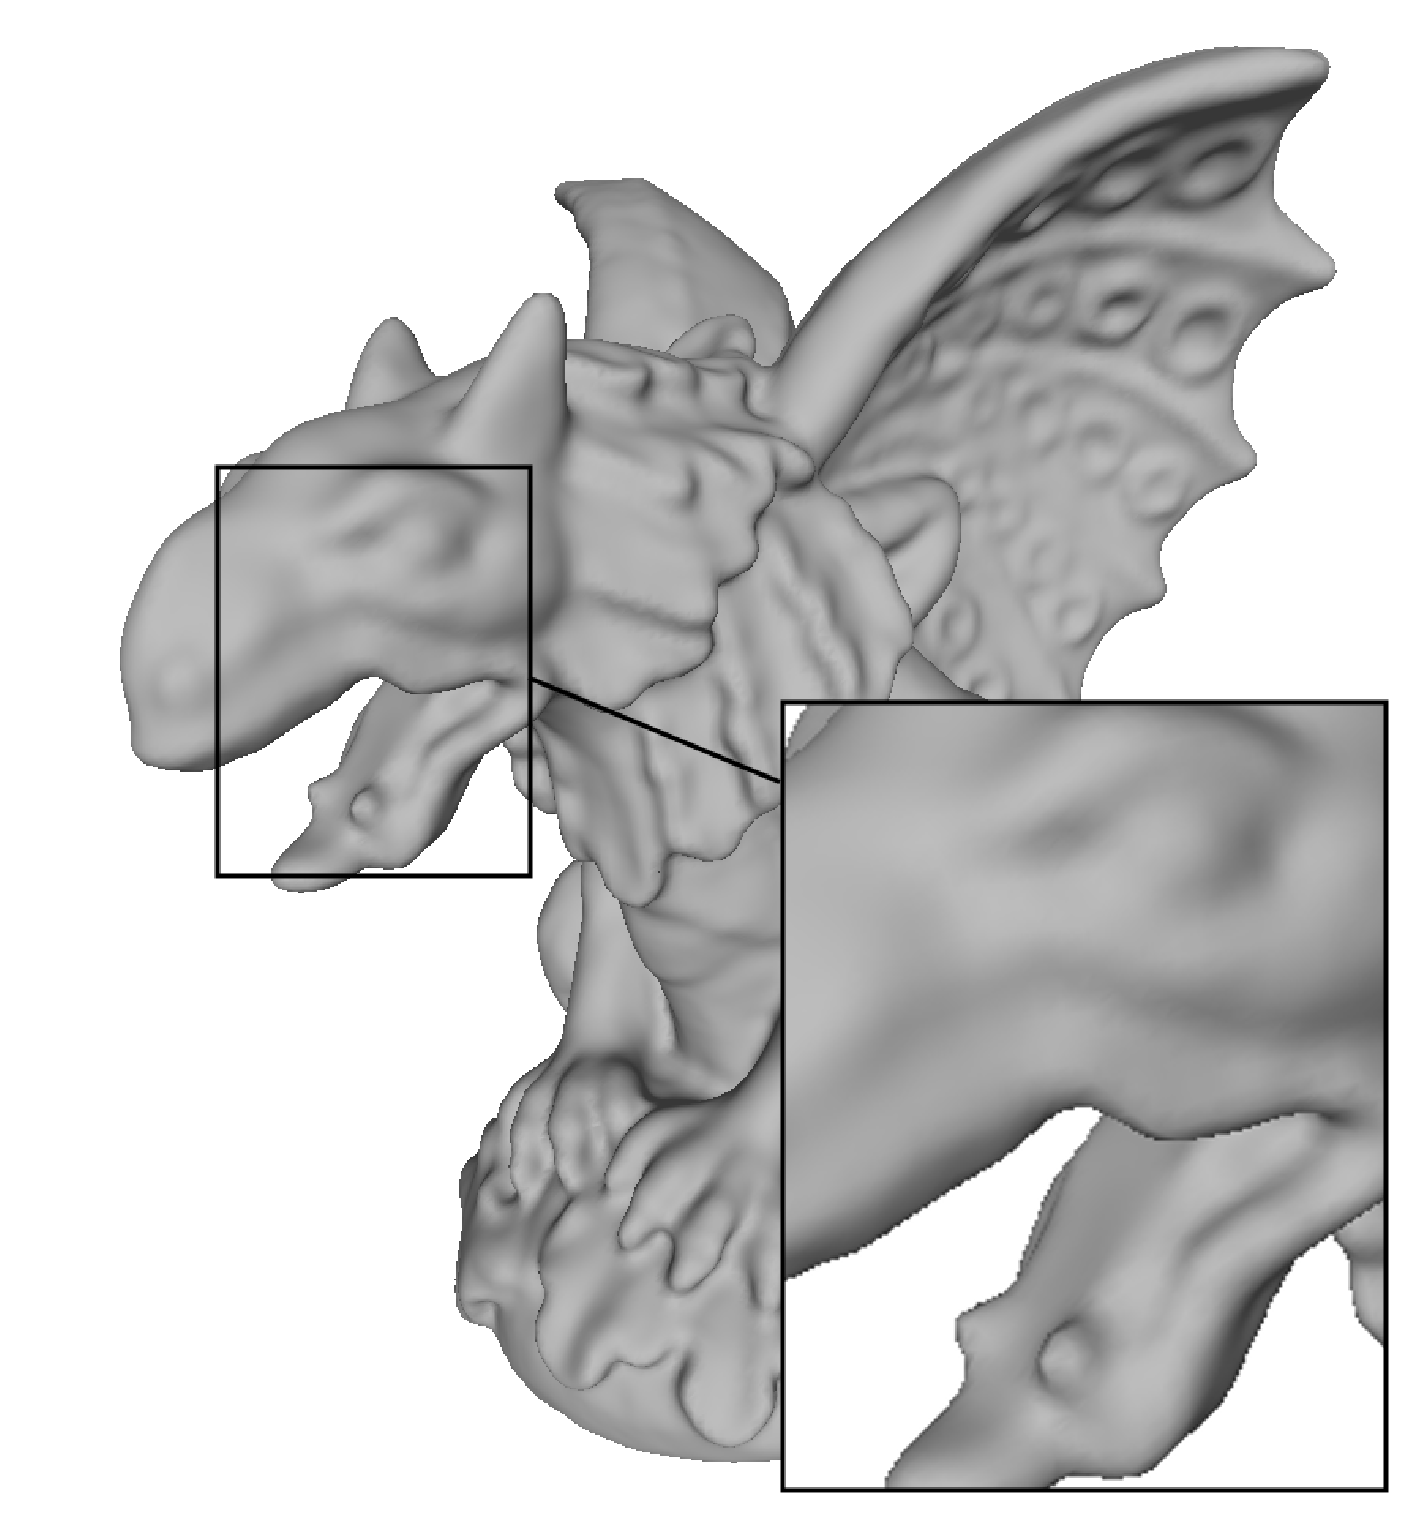
\includegraphics[width=0.49\linewidth,natwidth=750,natheight=750]{images/gargoyle/bcc4.eps} &
		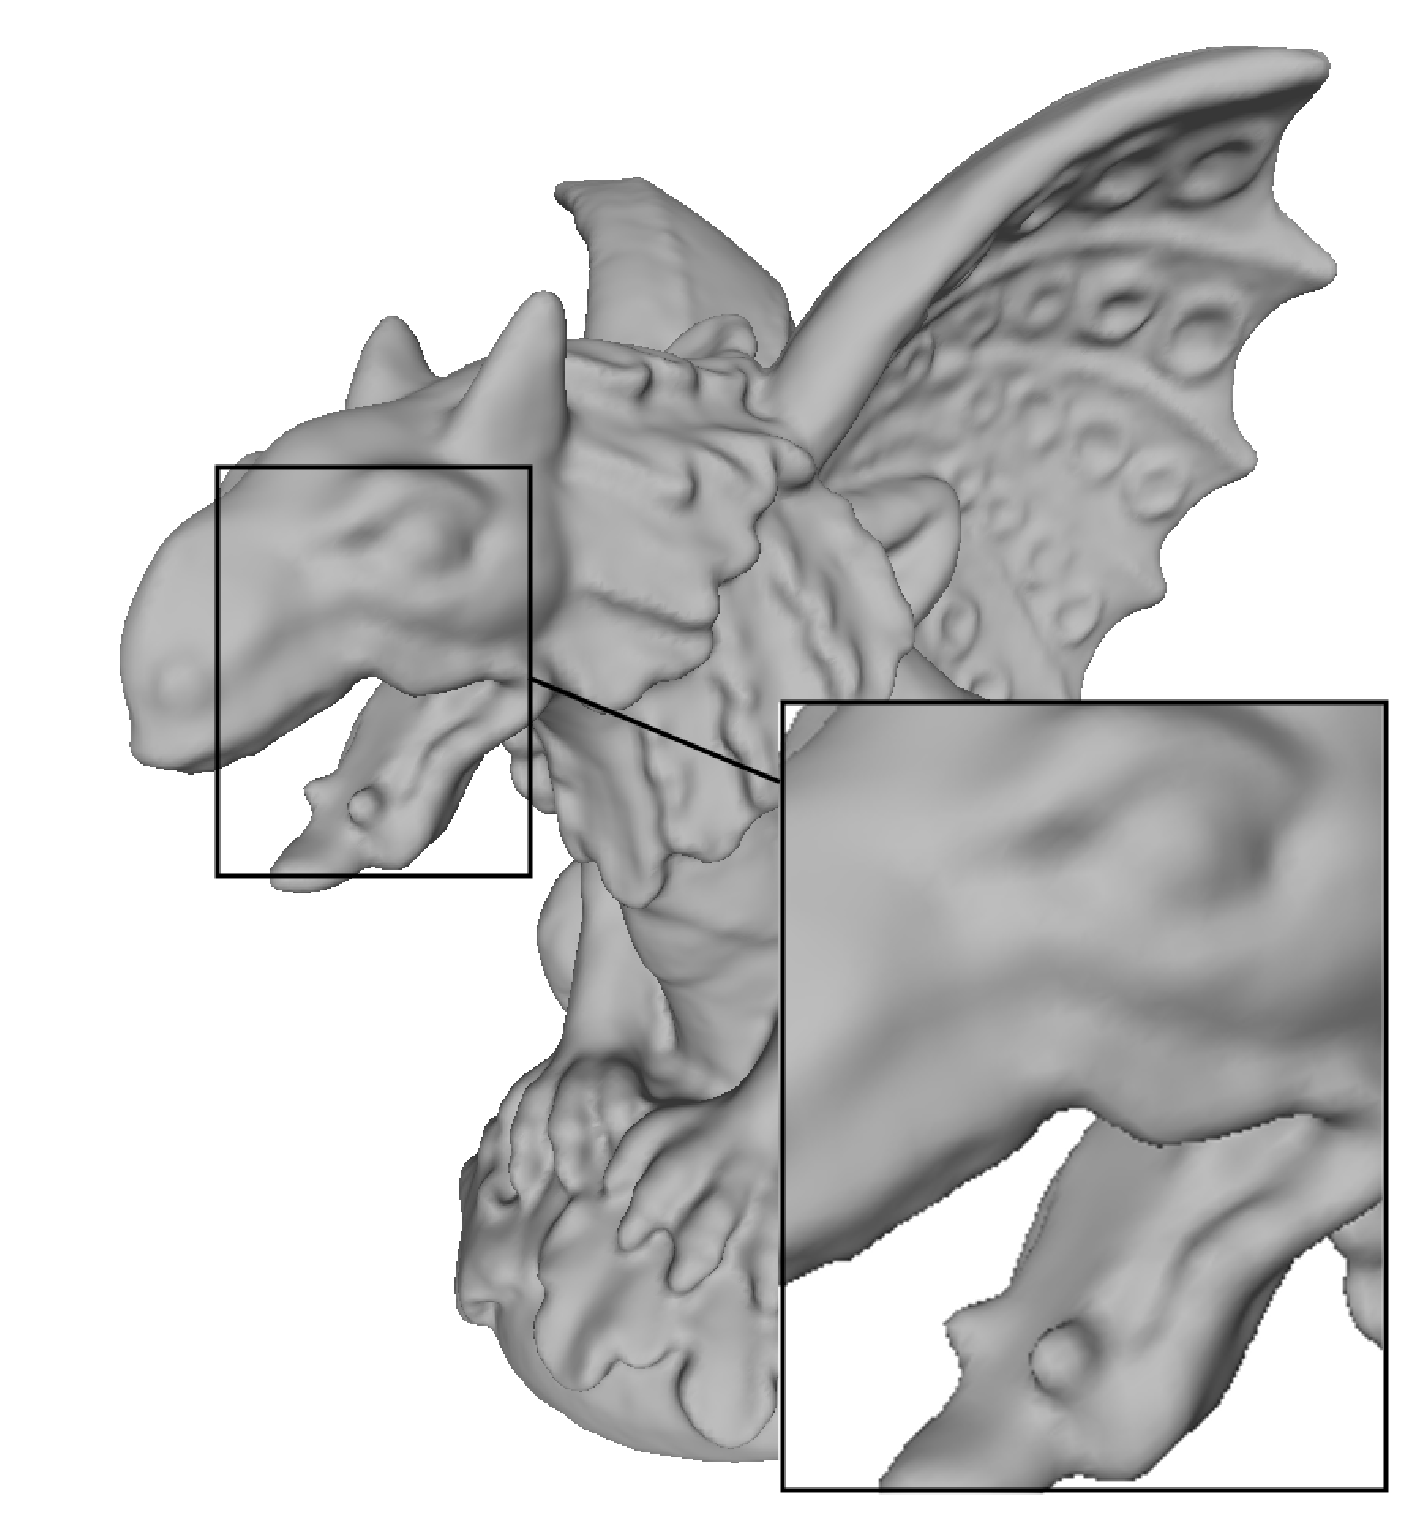
\includegraphics[width=0.49\linewidth,natwidth=750,natheight=750]{images/gargoyle/bcc4s.eps} \\
		BCC4 & BCC4 Shifted \\ 
		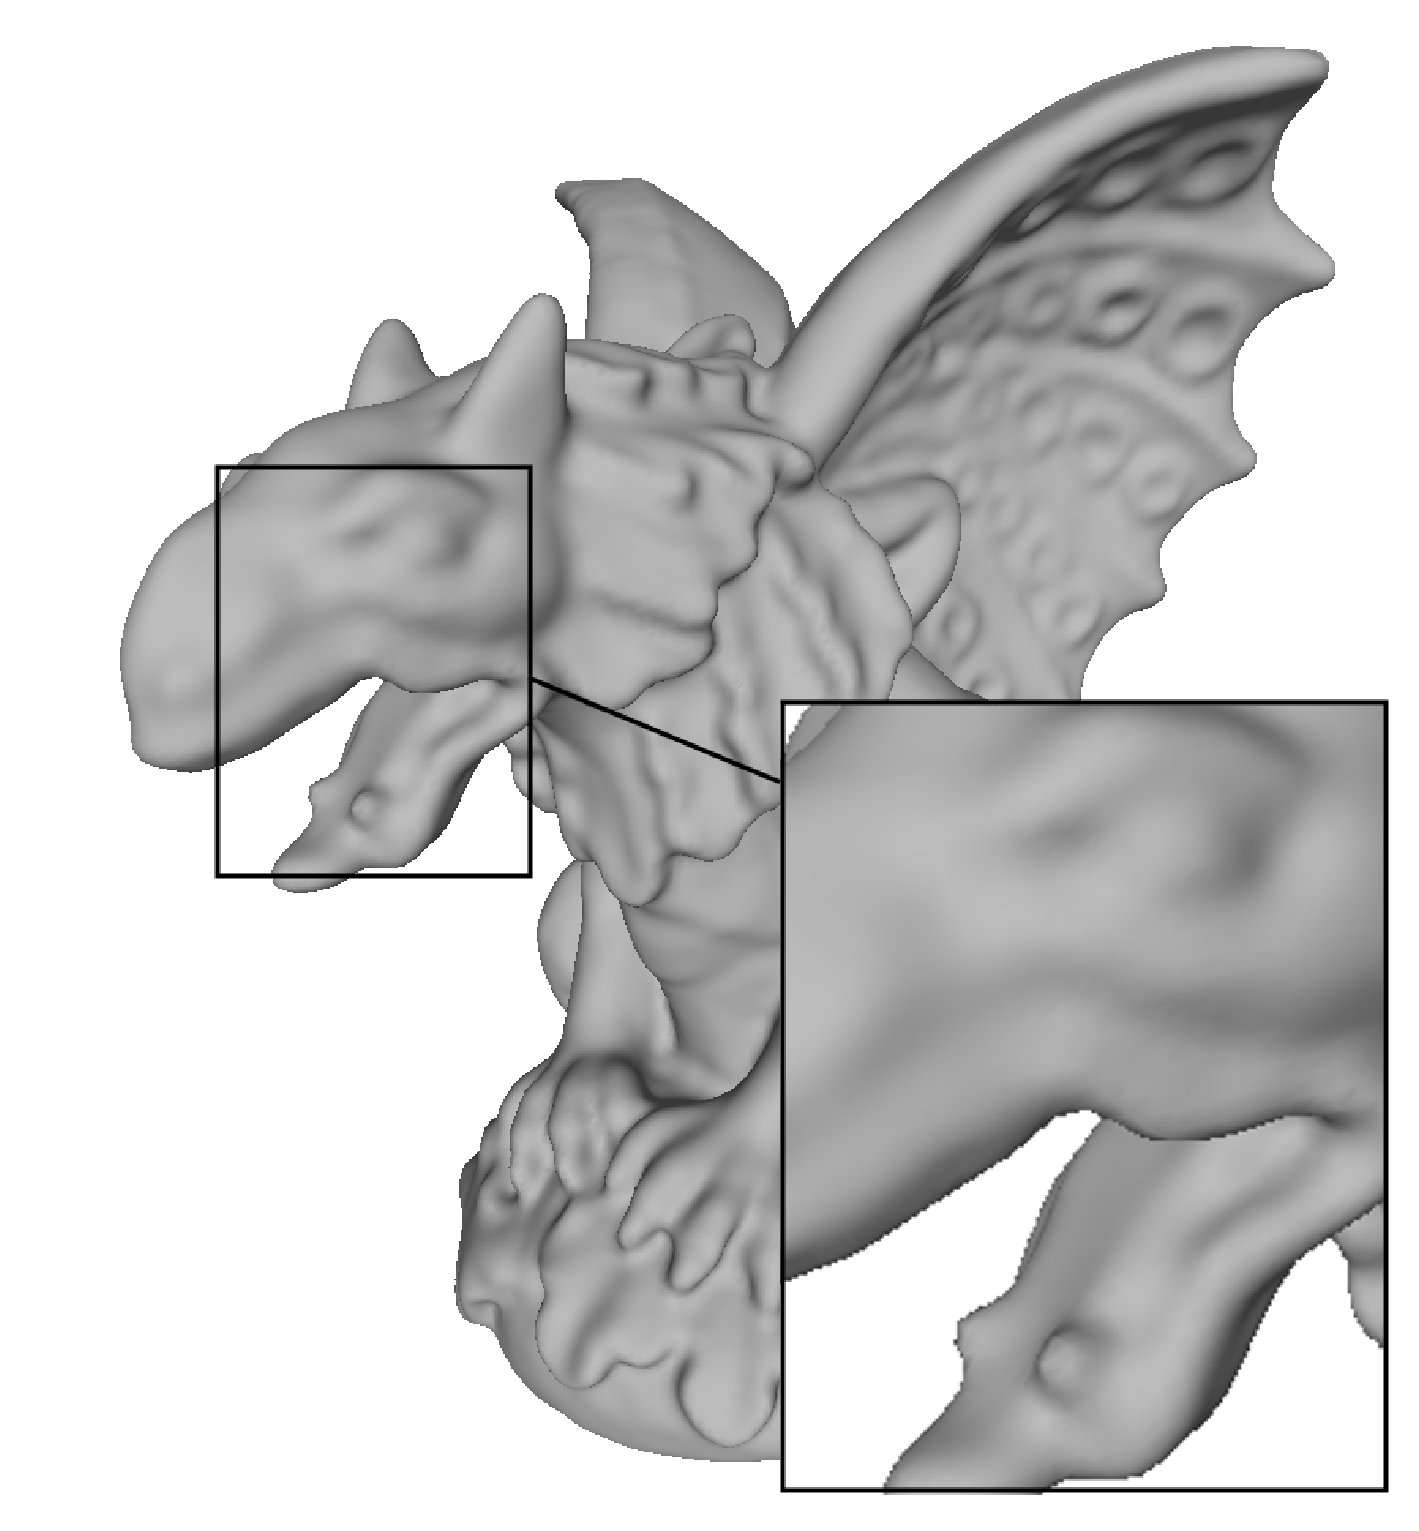
\includegraphics[width=0.49\linewidth,natwidth=750,natheight=750]{images/gargoyle/cc.eps} &
		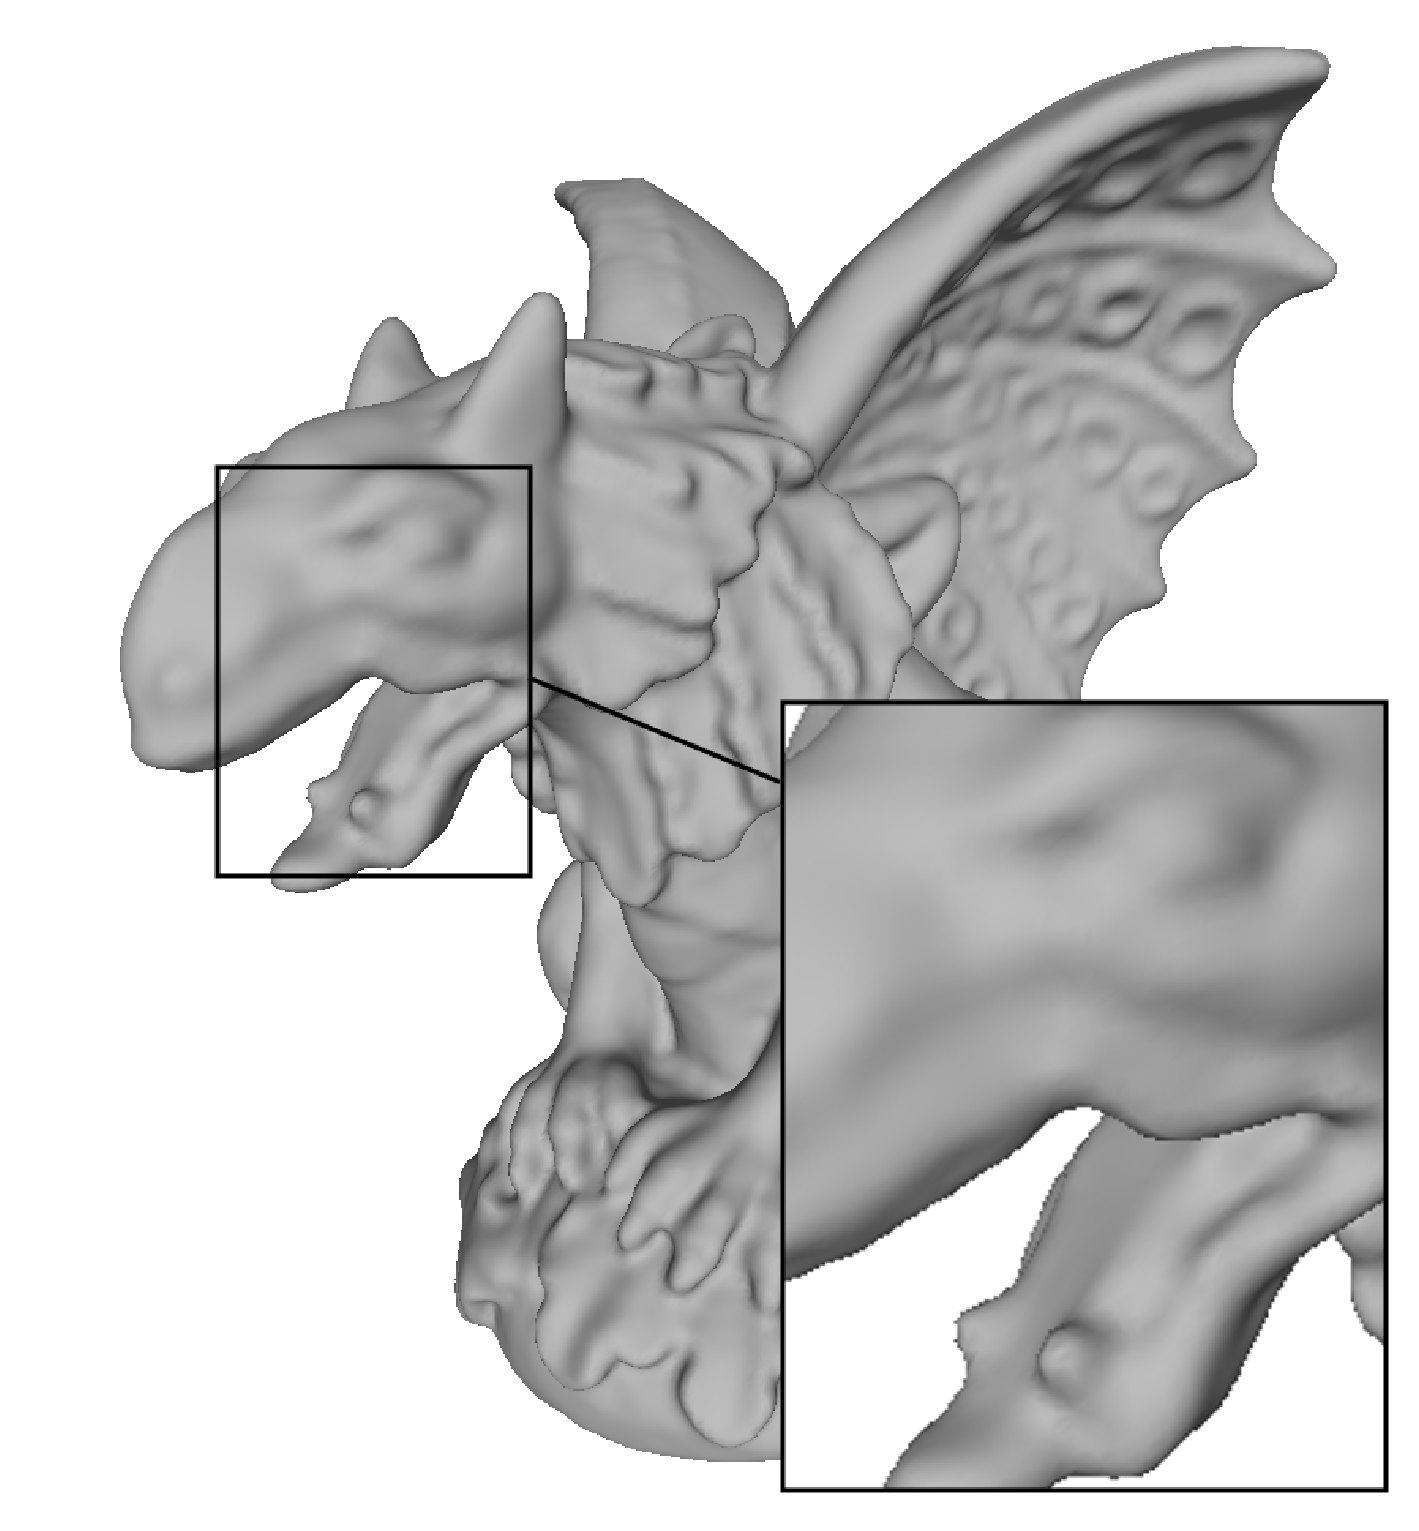
\includegraphics[width=0.49\linewidth,natwidth=750,natheight=750]{images/gargoyle/ccs.eps}  \\
		Cartesian & Cartesian Shifted 
	\end{tabular}
	\caption{A set of reconstructions on a $128^3$ Cartesian grid, $50\times50\times100$ BCC grid or an oct-tree depth of 7. Parameters were chosen as $\lambda_1 = 1\scint{2}$ and $\lambda_2 = 1\scint{-4}$. Comparing between the Cartesian and BCC reconstruction spaces, the BCC lattice seems to consistently outperform the Cartesian lattice beyond a resolution of $128^3$, moreover, the advantage of shifting the reconstruction space is apparent, specifically around the teeth and lips of the model.}
	\label{fig:r1}
\end{figure}

\begin{figure} 
	\centering
	\begin{tabular}{c c}
		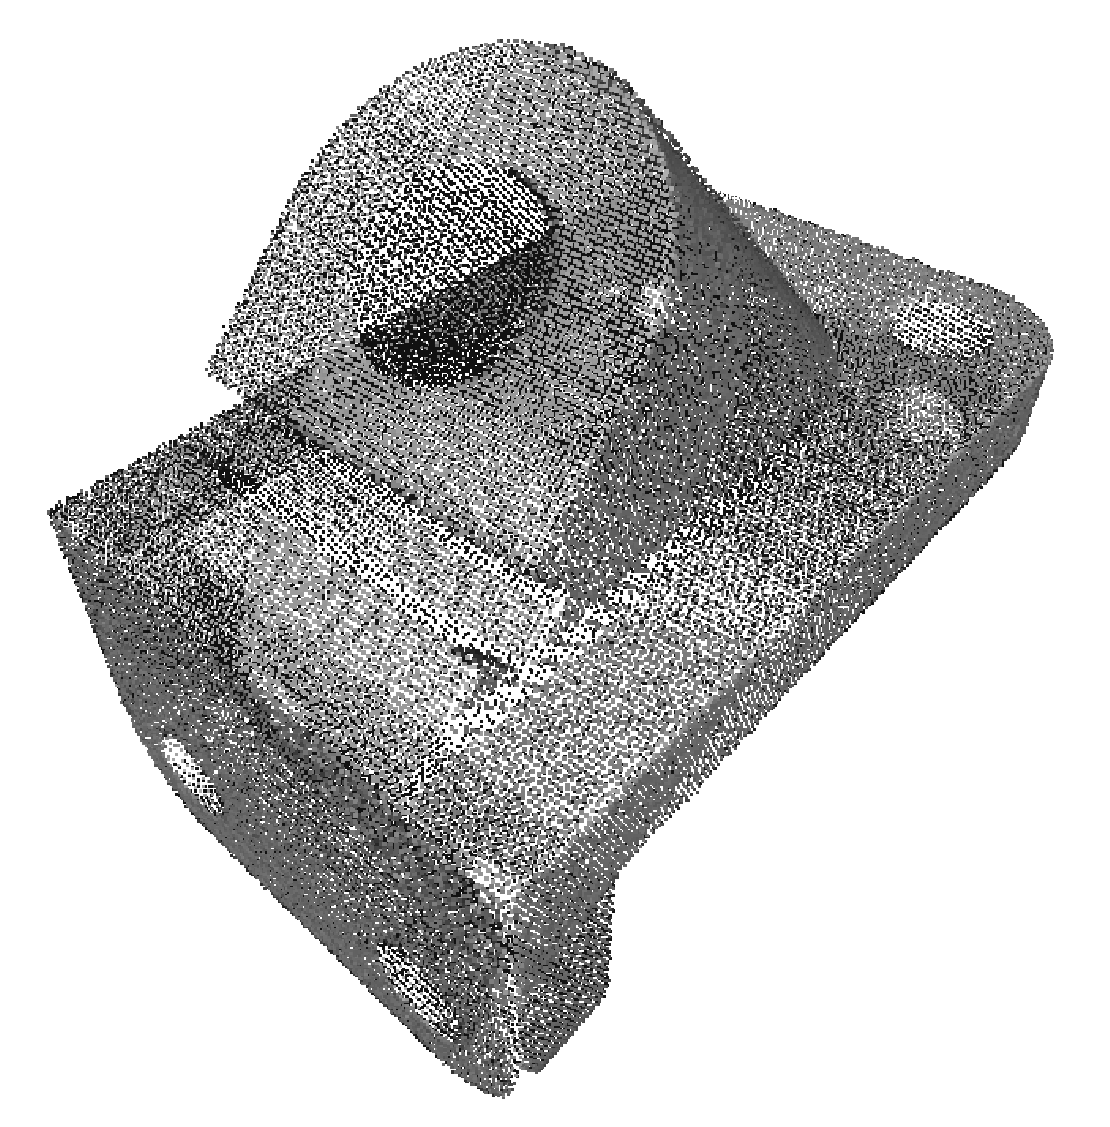
\includegraphics[width=0.48\linewidth]{images/robust/pointset.eps} &
		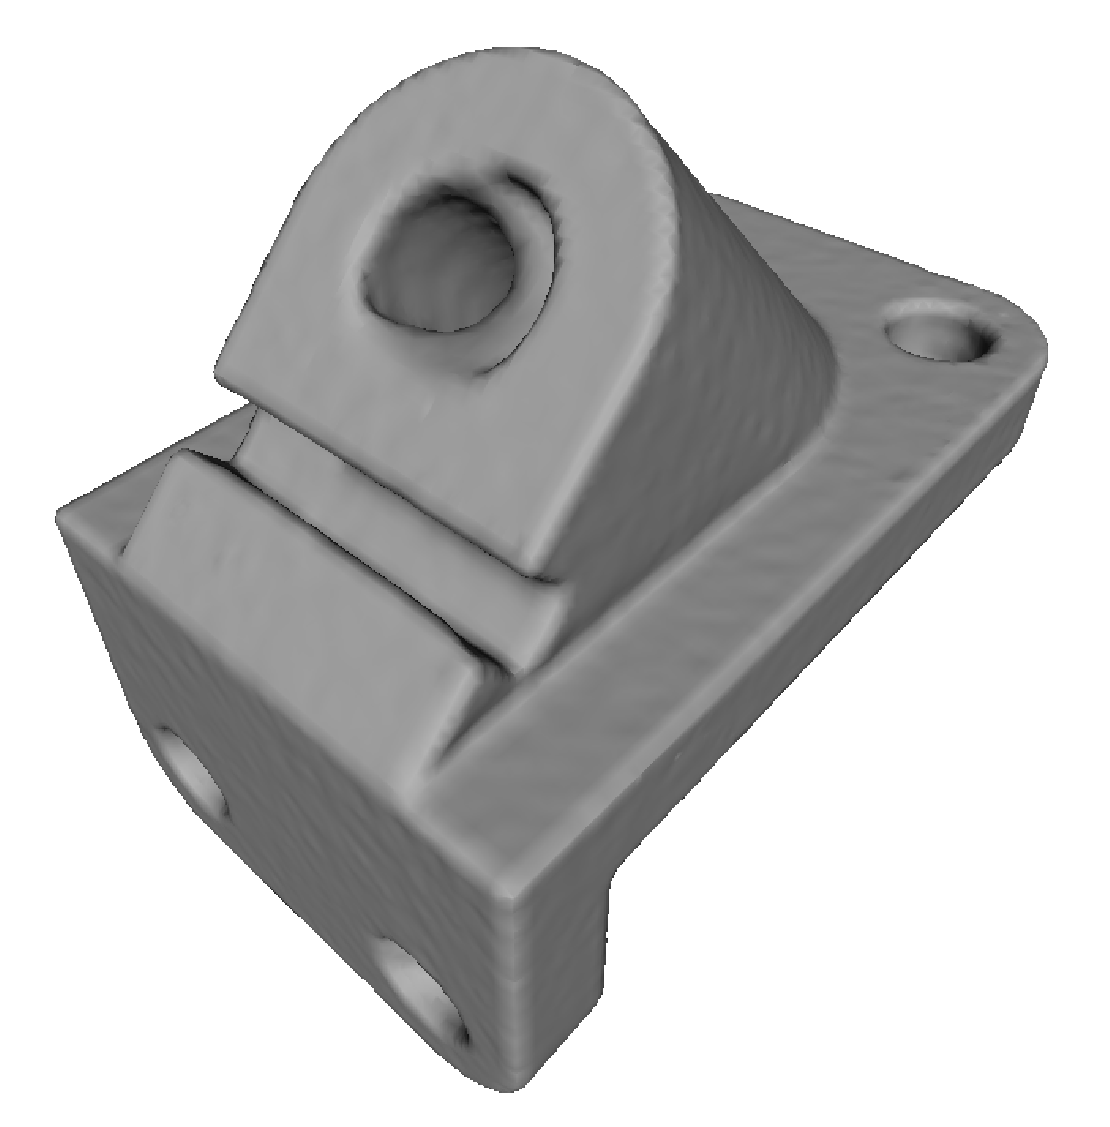
\includegraphics[width=0.48\linewidth]{images/robust/poisson.eps} \\
		Noisy Point-set & Screened Poisson  \\
		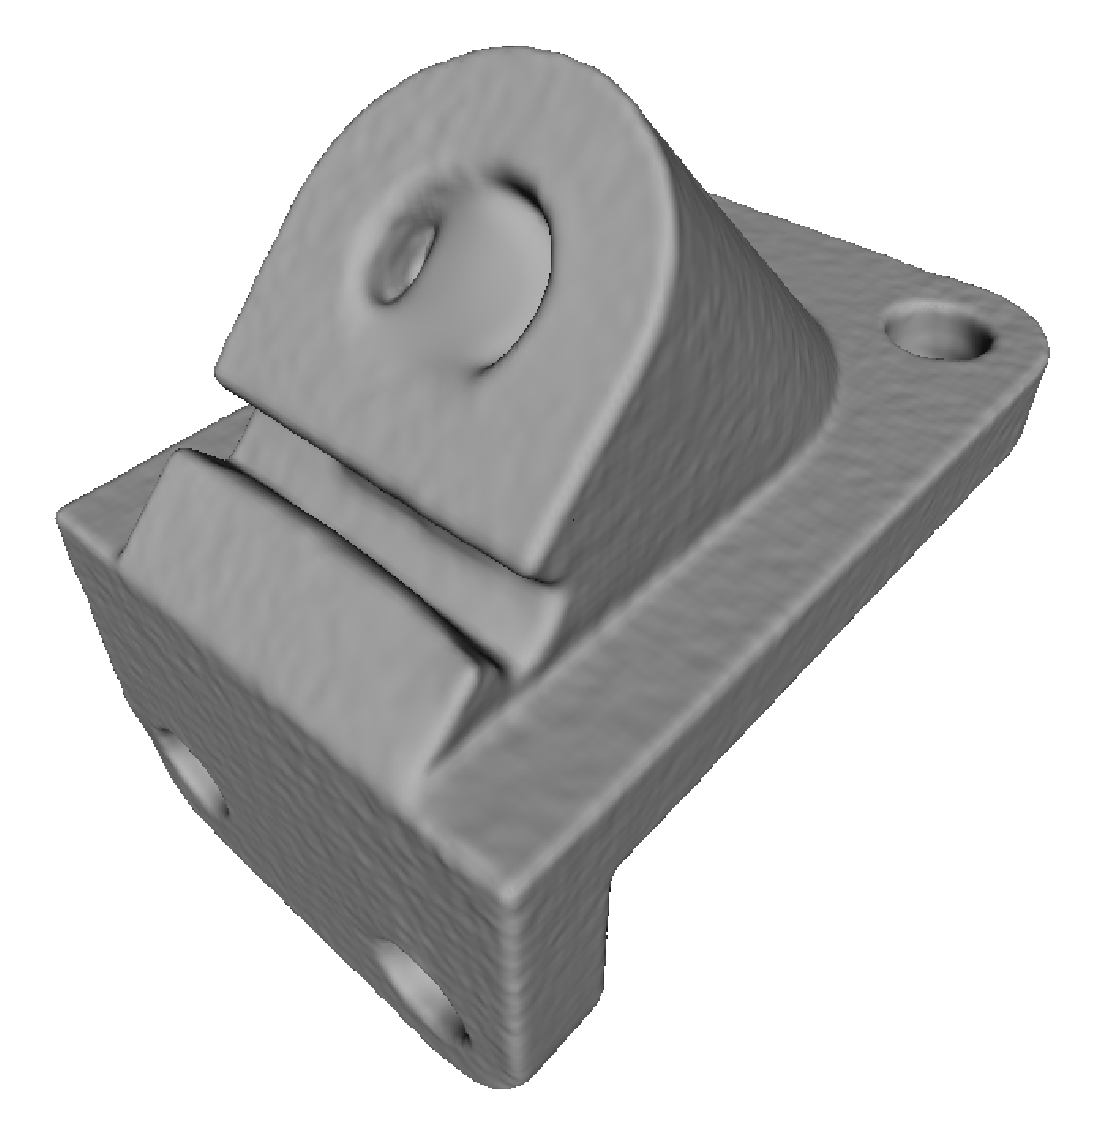
\includegraphics[width=0.48\linewidth]{images/robust/bcclowlambda.eps} &
		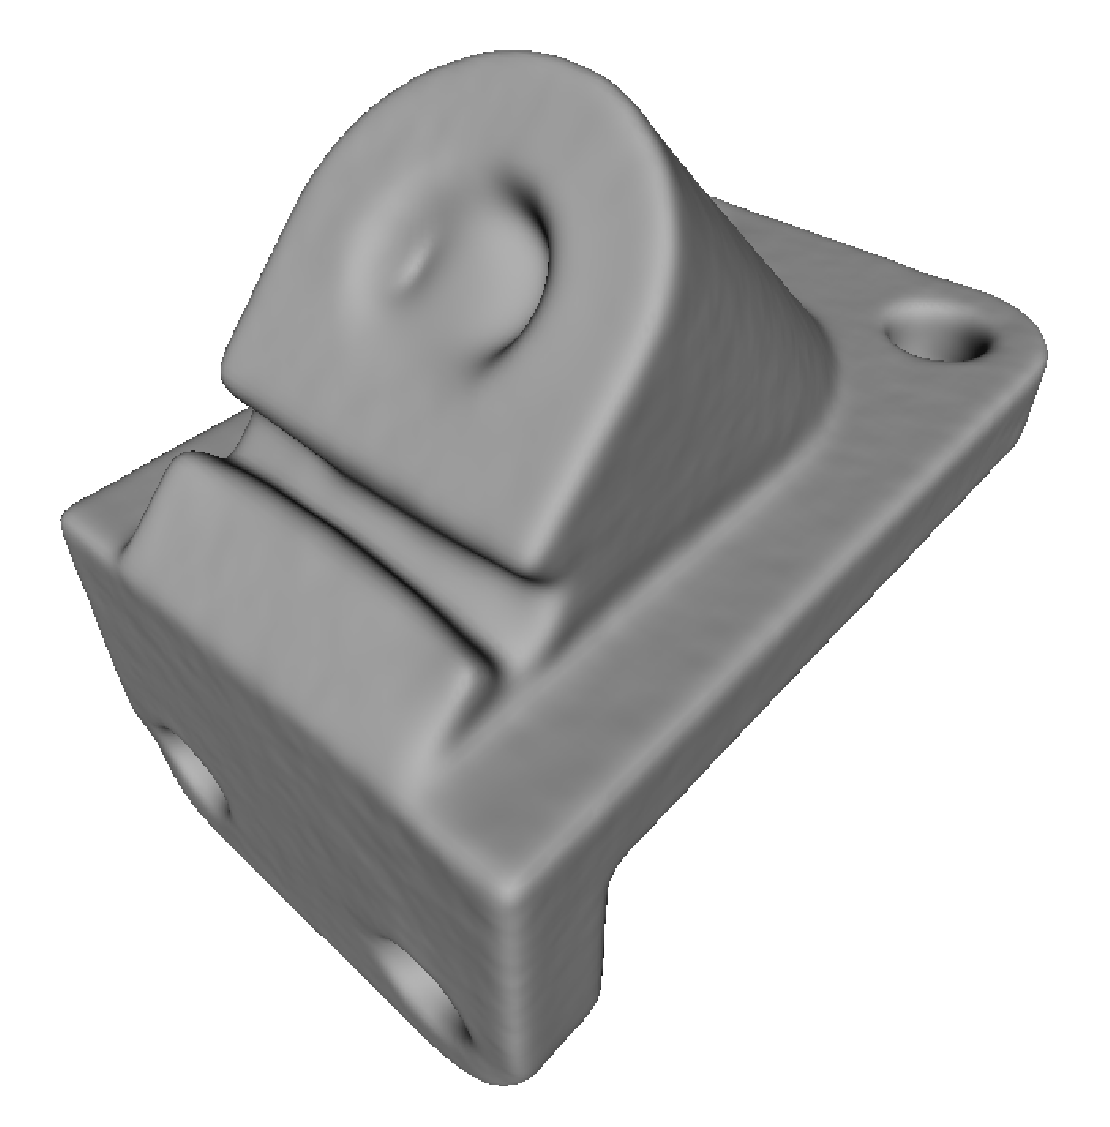
\includegraphics[width=0.48\linewidth]{images/robust/bccbiggerlambda.eps} \\ 
		BCCS $\lambda_2=5\scint{-5}$ & BCCS $\lambda_2 = 5\scint{-4}$ \\
	\end{tabular}
	\caption{Varying the smoothing parameter $\lambda_2$ allows us to smooth our noise from practical data sets $(\lambda_1 = 1\scint{2})$. The Screened Poisson method is able to more faithfully reconstruct the center hole of the Anchor model. Our method, however, is unable to infer the importance of the samples on the interior of the Anchor.}
	\label{fig:r2}
\end{figure}
